\section{Testes}
\label{sec:Testes}

\par Esta secção divide-se em duas subsecções, a primeira diz respeito a refactoring e identificação de Code Smells\footnote{Code Smell: característica do código fonte ou do programa que pode indicar um problema mais grave.}\cite{codeSmells1,codeSmells2} e a segunda prende-se com testes feitos á aplicação para testar a sua robustez.

\subsection{Refactoring e Code Smells}


\subsubsection{Devel::Cover}
\hfill\newline

\par Para realizar o processo de code coverage foi usado o módulo \textit{Devel::Cover}\cite{develCover}. Este módulo permite correr um programa com os respetivos argumentos e monitorizar que partes do código foram usadas ou não foram usadas, criando posteriormente um relatório em html que permite visualizar de uma forma mais clara o desempenho do programa.
\par Para utilizar o \textit{Devel::Cover} com o nosso programa e posteriormente criar o relatório pretendido basta correr os seguintes comandos pela ordem apresentada:
\begin{itemize}
	\item perl -MDevel::Cover signpdf\_cli.pl -u '+351 XXXXXXXXX' -p XXXX -infile teste.pdf -d
	\item cover
\end{itemize}

Após o programa terminar de executar podemos verificar que foi criada uma base de dados \textit{cover\_db} e que a informação da mesma foi compilada num relatório html.
O resultado de correr o teste\footnote{Note-se que a utilização do -d não é obrigatória mas foi usado para cobrir a maioria do código.} é apresentado em seguida:

\begin{figure}[H]

  \centering
  \captionsetup{justification=centering}

  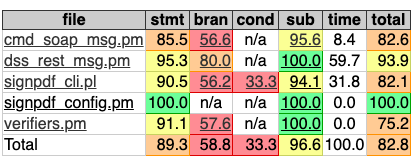
\includegraphics[scale = 0.25]{coverage1.png}
  
  \caption {Resultado de correr o programa utilizando o módulo Devel::Cover}

  \label{fig:coverage1}
\end{figure}


\par Analisando a imagem anterior, verificamos que existem várias colunas na tabela, cada coluna tem o seguinte significado da esquerda para a direita respetivamente: número de linhas do código utilizadas, nº de branches(if/else) utilizados\footnote{O número ótimo de branches utilizados é de 50\% uma vez que quando o código chega a um if then else segue apenas 1 dos caminhos possíveis, no entanto existem partes do código que possuem apenas um if ou que possuem sub-rotinas que não foram chamadas que possuem ifs, estes ifs contam para esta percentagem, fazendo o valor final subir ou descer respetivamente.}, percentagem das condições (as condições são compostas por elementos conjugados com as palavras \textit{and} e \textit{or}) avaliadas de forma positiva ou negativa, percentagem de sub-rotinas usadas, tempo em segundos que as sub-rotinas de cada ficheiro demoraram a executar.
\par Ao analisarmos os ficheiros para verificarmos que "statements" não estão a ser utilizados no código podemos verificar que estes se encontram todos dentro de condições if then else, sendo que como o programa correu bem, os statements não utilizados se encontram dentro dos else. Analisando a utilidade dos "statements" dentro de cada else constatamos que na sua maioria se tratam de comandos \textit{die} com informação sobre o porquê do programa ter sido interrompido naquele estágio, jutificando a sua permanência.


\par Passando agora á análise dos branches do programa, devemos analisar para cada ficheiro se os branches são necessários, ou seja se as condições para que se siga por cada um dos caminhos das biforcações se manifestam. Tomemos por exemplo o relatório referente ao ficheiro \textit{cmd\_soap\_msg.pm}.

\begin{figure}[H]

  \centering
  \captionsetup{justification=centering}

  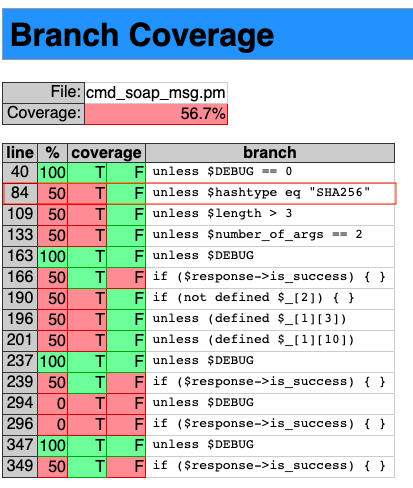
\includegraphics[scale = 0.25]{SOAPcoverage2.png}
  
  \caption {Relatório de branches do ficheiro cmd\_soap\_msg.pm}

\end{figure}

\par Após verificarmos a validade de cada branch, podemos observar que há um branch que não faz sentido porque verifica se um dado valor foi recebido como input dessa subrotina sendo que esse valor é passado de forma estática (esse branch foi assinalado a vermelho para facilitar o seu reconhecimento). Podemos então apagar esse branch uma vez que não tem utilidade no código. O mesmo processo foi aplicado a cada ficheiro, no entanto optou-se por não se mostrar visto que o tratamento é homólogo e não houve mais nenhum caso de uma condição desnecessária.

\par Podemos ainda ver, na figura\ref{fig:coverage1}, que existe uma condição no código. O módulo Devel:Cover cria também um relatório para as condições do programa como se pode ver na imagem abaixo.

\begin{figure}[H]

  \centering
  \captionsetup{justification=centering}

  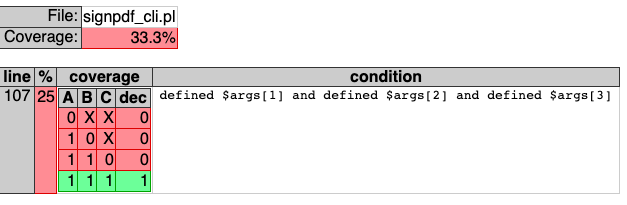
\includegraphics[scale = 0.25]{condition.png}
  
  \caption {Relatório de condições do ficheiro signpdf\_cli.pl}

\end{figure}

Podemos verificar que são mostradas as vária verificações que podem ser levadas a cabo e os respetivos resultados. Estes resultados são todos possíveis porque até aquele ponto não existe verificação se os 3 elementos que o cliente tem de fornecer ao programa são realmente fornecidos.
\par Concluida a verificação de existência de código inútil, confuso, muito extenso ou duplicado confirma-se que o único problema encontrado foi a existência do if que fazia a verificação de um elemento estático do código.


\subsubsection{Perl::Critic}
\hfill\newline

\par Após serem removidos os code Smells do código usou-se uma biblioteca chamada \textit{Perl::Critic}\cite{perlCritic} que avalia o código fonte de acordo com as diretrizes do livro Perl Best Practices\cite{bestpractices}, além de avaliar outras métricas, como a complexidade ciclomática. Este módulo permite escolher 5 tipos de severidade de problemas no código, podendo as falhas mais severas representar problemas que permitam que um utilizador mal intencionado se aproveite do nosso programa e as falhas mais ligeiras apenas questões de legibilidade do código. Por esta razão começamos por definir uma severidade de grau 4, desta forma apenas foram apresentados os erros mais graves, de severidade 5, a vermelho e os segundos mais graves, de severidade 4, a laranja\footnote{Por questões de simplicidade de apresentação apenas é apresentado o resultado da aplicação do módulo ao ficheiro signpdf\_cli.pl, no entanto ressalva-se que o mesmo processo foi aplicado aos restantes ficheiros do programa.}.

\begin{figure}[H]

  \centering
  \captionsetup{justification=centering}

  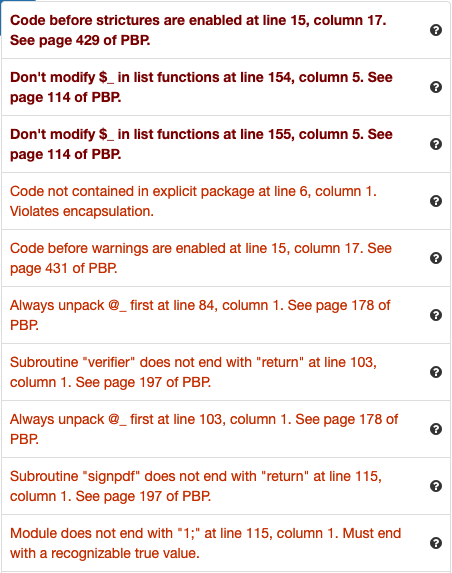
\includegraphics[scale = 0.3]{critic1.png}
  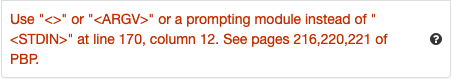
\includegraphics[scale = 0.3]{critic2.png}
  
  \caption {Relatório \textit{Perl::Critic} de gravidades 4 e 5 do ficheiro signpdf\_cli.pl}

\end{figure}

\par As 3 primeiras notificações apresentadas correspondem a problemas críticos no código perl que foram resolvidos adicionando, após a adição do último módulo necessario, \textit{use strict;} para a primeira notificação e para as restantes duas bastou remmover o map que estava a ser usado para modificar uma lista de certificados aplicando um regex substituindo-o pela sub-rotina \textit{apply()} do módulo \textit{List::MoreUtils}\cite{perllist}. As restantes notificações possuem severidade 4. 
\par A primeira notificação refere-se á não identificação do código atual como um package, notificação essa que foi prontamente resolvida indicando na primeira linha do código \textit{package signpdf\_cli;}. A segunda notificação desapareceu com a adição do "use strict;" utilizado para remover a primeira notifiação de severidade 5.
\par Duas das notificações referiam que se trata de uma boa prática copiar o array recebido por uma sub-rotina para uma variável extra e utilizar esta, uma vez que caso o array original seja alterado dentro da sub-rotina, essa alteração \mbox{refletir-se-á} na sub-rotina que a invocou. Adicionalmente 3 outras notificações foram resolvidas adicionando \textit{return 1;} ao final de todas as sub-rotinas que ainda não o possuiam e \textit{1;} no final do ficheiro, visto que os ficheiros em perl devem acabar com um valor de verdade.
\par Por fim o uso de \textit{<STDIN>} foi substituido pelo uso da sub-rotina \textit{prompt} pertencente ao módulo \textit{IO::Prompt}\cite{ioPrompt}.

Como todas as notificações para uma análise de gravidade 4 pareciam importantes, decidi diminuir o filtro de gravidade da análise do ficheiro para 3 e o resultado obtido pode-se ver na imagem abaixo.

\begin{figure}[H]

  \centering
  \captionsetup{justification=centering}

  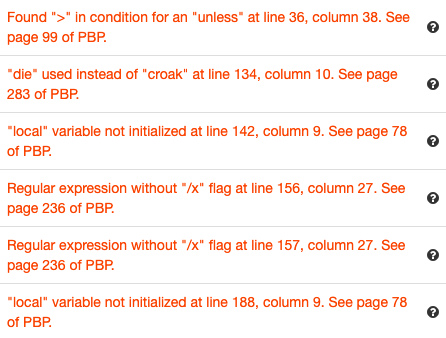
\includegraphics[scale = 0.4]{critic3.png}
  
  \caption {Segundo relatório \textit{Perl::Critic} de gravidade 3 do ficheiro signpdf\_cli.pl}

\end{figure}
\par Estes erros são meramente para melhorar a simplicidade aciclomática do código, ou a legibilidade do mesmo, por esse motivo apliquei as mudanças requeridas ao ficheiro.
\par A primeira notificação referia que ao usar o simbolo de > dentro de um unless implicava uma dupla negativa (trata-se de uma questão de sacrificar velocidade de execução do código por legibilidade), assim foi modificado o código, trocando o unless por um if tornando o código mais eficiente.
\par A segunda notificação apenas pretende assinalar que quando nos deparamos com um erro de input por parte do utilizador, não devemos usar o comando \textit{die} que serve para reportar erros da aplicação mas o comando \textit{croak} que serve explicitamente para assinalar que o erro foi de terçeiros não da aplicação.
\par A terceira e quinta notificações dizem respeito á legibilidade do código, apesar de uma variável declarada á qual não se atribui valor ser indefinida por defeito, devemos indicar explicitamente isto atribuindo-lhe o valor \textit{undef}.\newline
\par Por fim é referido que a expressão \textit{s/\textbackslash s*-----\textbackslash s*BEGIN CERTIFICATE\textbackslash s*-----\textbackslash s*//} é demasiado grande e dificil de ler e deve ser dividida para que se possam acrescentar comentários a cada parte da divisão para que se perceba o que se está a pretender obter com aquela parte do regex, no entanto, este erro deve-se á adição dos \textit{\textbackslash s*} algo que a meu ver não influencia a legibilidade, adicionalmente separar este regex tornalo-ia mais confuso do que está atualmente uma vez que este pretende representar uma string relativamtne compacta sendo os \textit{\textbackslash s*} adicionados apenas uma medida de precaução. Pelos motivos enunciados anteriormente estes avisos foram ignorados.
\hfill\newpage

\subsubsection{Test::Vars}
\hfill\newline

\par Adicionalmente, foi criado um script perl chamado \textit{tester.pl} que utiliza o módulo \textit{Test::Vars}\cite{testVars} para garantir que não existem variáveis por usar no programa. O resultado de correr este script sobre os ficheiros do programa é o seguinte:

\begin{figure}[H]

  \centering
  \captionsetup{justification=centering}

  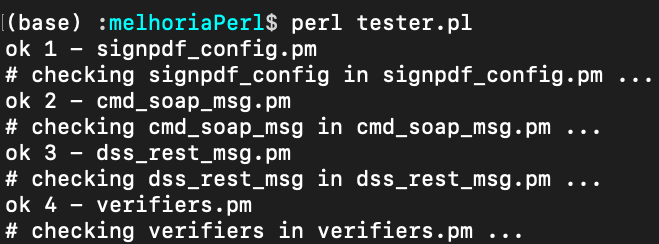
\includegraphics[scale = 0.25]{testvars.png}
  
  \caption {Verificação de variáveis não utilizadas nos ficheiros do programa}

\end{figure}
\par Como se pode verificar não existe a presença de variáveis por utilizar nos ficheiros do programa.


\subsubsection{SonarQube}
\hfill\newline

\par Após todo o trabalho levado a cabo para corrigir qualquer falha no código do programa, utilizei o SonarQube\cite{sonarQube} com uma extensão para Perl\cite{perlSonarQube} para confirmar mais uma vez que o código está de facto bem escrito e não possui duplicações ou outros problemas. O resultado de correr este programa de validação e deteção de Code Smells sobre o nosso programa pode ser visualiado na figura a baixo apresentada.

\begin{figure}[H]

  \centering
  \captionsetup{justification=centering}

  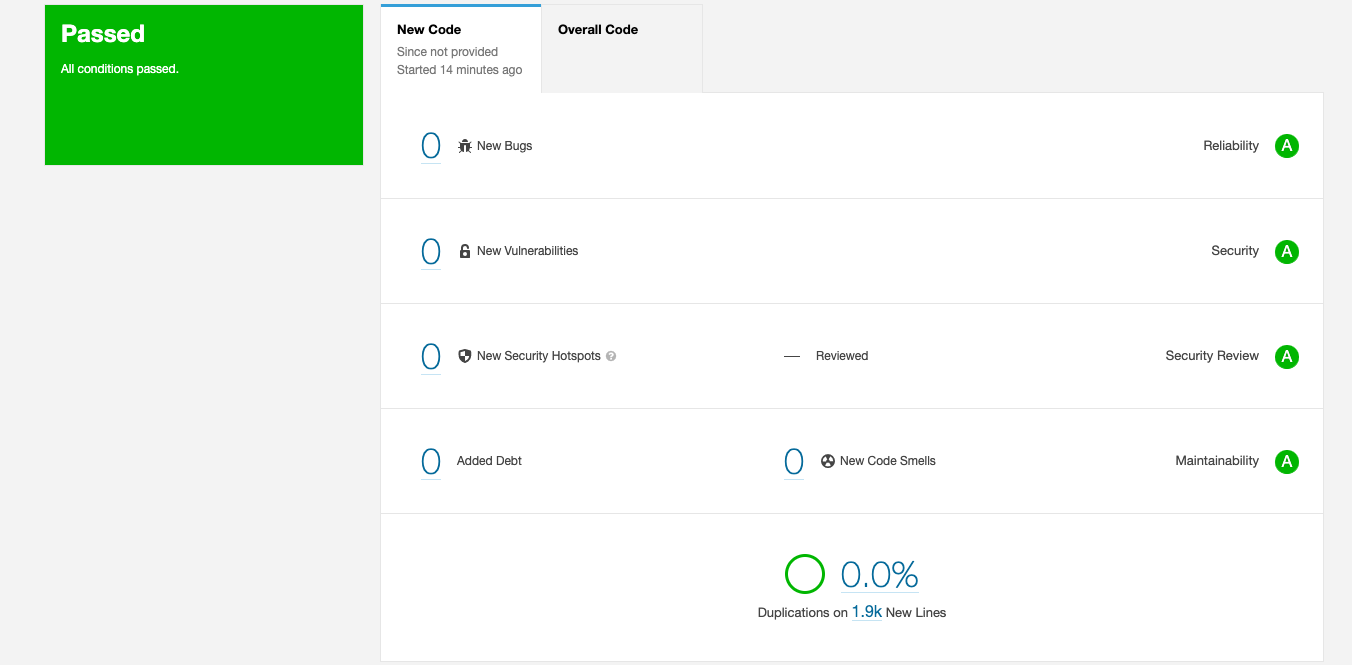
\includegraphics[scale = 0.25]{sonarQube.png}
  
  \caption {Relatório gerado pelo SonarQube sobre todos os ficheiros do programa}

\end{figure}

\par Claramente o programa não possui mais code Smells a serem retirados. Adicionalmente podemos verificar que, de facto, termos utilizado severidade de nivel 3 na análise recorrendo ao módulo \textit{Perl::Critic} foi a escolha certa uma vez que o addOn usado no SonarQube para verificar o código perl apresenta uma utilização refinada de vários módulos\cite{develCover,perlCritic} e regras de livros perl\cite{codeSmells2,livro1,livro2,livro3,bestpractices}. 

\subsection{Testes}

\par Para realizarmos testes sobre a aplicação, temos de verificar de que forma a podemos comprometer. A forma que temos de tentar realizar um ataque é através da inserção de inputs maliciosos, que podem ser introduzidos quando se passam argumentos no inicio programa ou no seu decorrer ou então quando o programa recebe uma resposta do servidor. Note-se que apesar de os inputs serem recebidos, todos sem exceção são enviados a alguma sub-rotina do módulo \textit{verifiers.pm} para verificação. Assim, para testar a robustez do programa basta tentar obter um resultado inesperado nos testes do módulo \textit{verifiers.pm} quando este deveria alertar para um erro de input, para este fim realizamos um fuzzing com recurso ao módulo \textit{Test::LectroTest}\cite{testelectro}. Este módulo permite definir propriedades que definem o tipo de inputs a passar ás funções a testar e o tipo de resposta esperado para esses inputs, adicionalmente, podemos criar uma mensagem informativa sobre a propriedade que está a ser testada.
\par Cada um dos inputs das propriedades supramencionadas pode ser definido como um tipo de variável, sendo que o módulo gerará esse input automaticamente ou alternativamente é possível criar um gerador para o input declarado, isto dá jeito quando, por exemplo, ao invés de uma string aleatória queremos uma string que contenha apenas letras minúsculas.
\par Foi por isso criada uma propriedade para cada verificação individual realizada no módulo \textit{verifiers.pm} que é testada sobre os inputs fornecidos e para cada input foi criado um gerador que permite testar um parte da sub-rotina de verificação. Tomemos por exemplo os geradores, a propriedade definida e e validação dos outputs da sub-rotina \textit{valid\_response()}. O primeiro passo para conseguirmos definir uma propriedade sobre esta é entender o seu funcionamento.
\begin{figure}[H]

  \centering
  \captionsetup{justification=centering}

  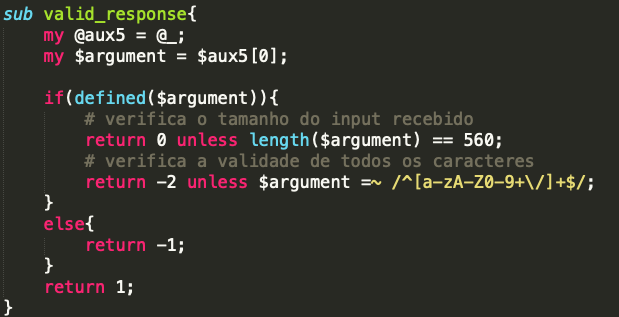
\includegraphics[scale = 0.25]{validateResponse.png}
  
  \caption {Sub-rotina valid\_response()}

\end{figure}
\par Esta começa por verificar se o valor recebido está definido, caso não esteja devolve -1, o que permitirá ao corpo principal do programa escrever a mensagem informativa: \textit{"Response not defined!"} antes de terminar. Caso a variável esteja definida temos 3 opções, a primeira é a variável não ter o comprimento certo, isto pode ser resultado de uma interseção da mensagem por parte de terceiros e consequente alteração do tamanho da mesma quer por truncação quer por adição, a sub-rotina prontamente devolve o código de erro 0 que permite mostrar ao utilizador a mensagem \textit{"Illegal length found on Response!!"} . A segunda hipótese prende-se com a alteração dos valores da mensagem de forma a inserir código com fins nefastos, assim é realizada uma verificação que garante que os caracters da mensagem são todos de base 64, caso não sejam esta sub-rotina devolve o valor de erro -2 que permite mostrar a seguinte mensagem de erro ao utilizador: \textit{"Wrong charaters on Response!!"}. Por fim temos a terçeira opção que assume que ao passar pelas várias validações o input é o original e está correto e portanto devolve o código 1 que permite que o programa avance. Assim, o nosso objetivo é fornecer um input que supostamente deva falhar uma verificação ou passar todas e cujo código devolvido não seja o esperado. O código desenvolvido com este intuito apresenta~se em seguida.


\begin{figure}[H]

  \centering
  \captionsetup{justification=centering}

  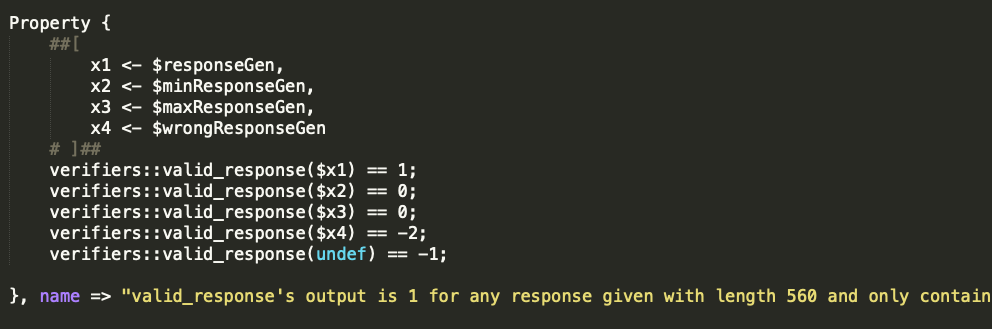
\includegraphics[scale = 0.3]{validateResponseTester.png}
  
  \caption {Propriedade que testa outputs da sub-rotina valid\_response()}

\end{figure}

Com se pode ver na imagem acima temos dentro da propriedade 4 inputs declarados com a sintax do módulo \textit{Test::LectroTest} e para cada input temos uma chamada á sub-rotina a testar. Os geradores destes inputs são apresentados em seguida bem como qual a propriedade que o input gerado pretende testar.
\begin{enumerate}
	\item String( charset=>"A-Za-z0-9+/", length=>[560])
	\par Este gerador gera uma mensage em base 64 que deve passar todos os testes de validação de input. A validação deve retornar sempre 1.\newline
	\item String( charset=>"A-Za-z0-9+/", length=>[561,])
	\par Este gerador gera mensagens cujos caracters são válidos em base 64 mas cujo tamanho é superior ao esperado. A validação deve retornar sempre 0.\newline
	\item String( charset=>"A-Za-z0-9+/", length=>[1,559])
	\par Este gerador gera mensagens cujos caracters são válidos em base 64 mas cujo tamanho é inferior ao esperado. A validação deve retornar sempre 0.\newline
	\item String( charset=>"[\&\%\$\#@"!?',;.:-\_ªº\textasciitilde\^{}\textbackslash\textbar]", length=>[560])
	\par Este gerador gera mensagens cujos caracters são inválidos em base 64 mas cujo tamanho é o esperado. A validação deve retornar sempre -2.
\end{enumerate}

Adicionalmente testaram-se também as respostas da validação a um input indefinido que, como previsto, retornou -1.

\par O mesmo tipo de raciocinio foi aplicada a cada sub-rotina do módulo \textit{verifiers.pm} e, no fim, as propriedades desenvolvidas foram aplicadas 10000 vezes, ou seja um número de vezes significativo para minimizar as hipóteses de terem sido gerados apenas inputs que favoreçam o intuito de cada propriedade e as avaliem como corretas. O resultado apresenta-se em baixo.


\begin{figure}[H]

  \centering
  \captionsetup{justification=centering}

  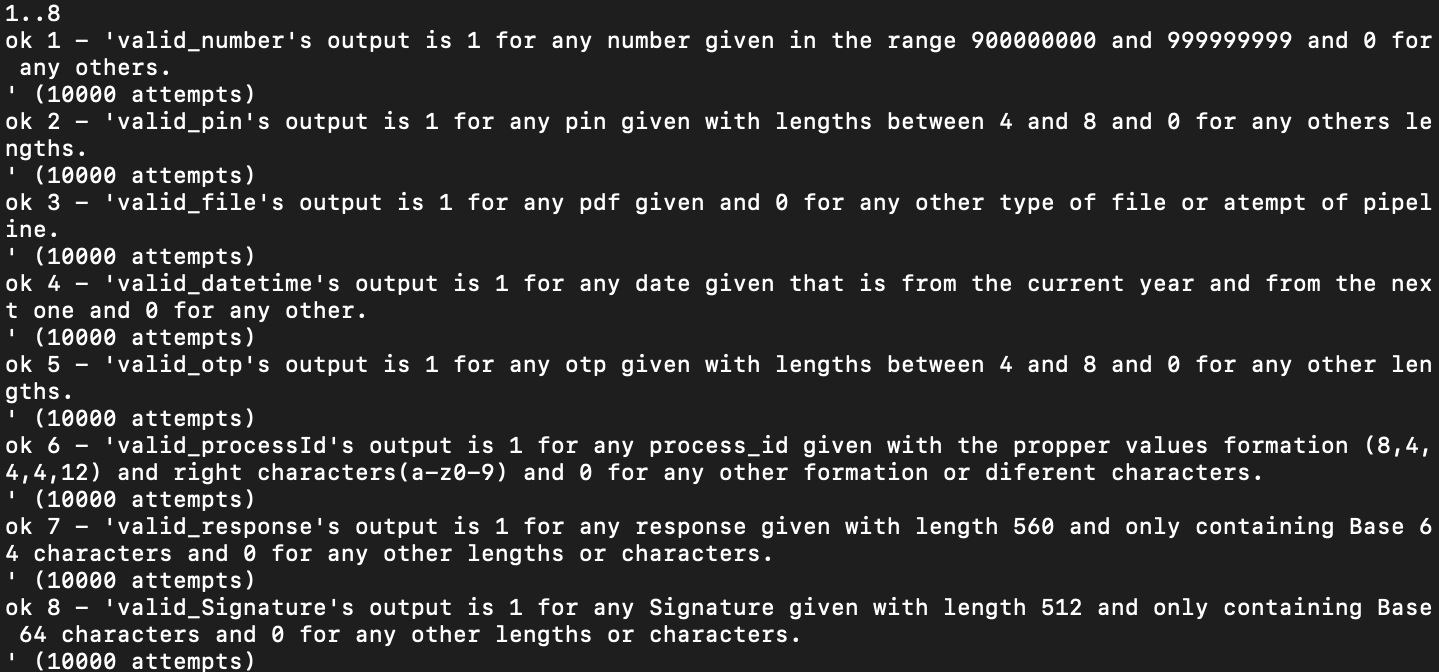
\includegraphics[scale = 0.25]{validations.png}
  
  \caption {Resultado das 10000 verificações utilizando cada uma das propriedades definidas}

\end{figure}



